\Chapter{Témaköri felvezetés}

\Section{A darts bemutatása}

A darts Angliából származó játék és sport, melynek a lényege hogy apró nyilakkal eltaláljuk a céltábla különböző pont értékű szektorait. A táblán összesen 20 plusz 1 szektor található meg, a 20 szektor értéke értelemszerűen 1-től 20-ig határolható be, de táblán belül megtalálható még két gyűrű is, a belső gyűrű amelyet, ha eltálunk akkor az adott szektor értékének a háromszorosát érjük el egy dobással, a külső gyűrű eltalálásával pedig a dobás szektor értékének kétszerese. A plusz 1 szektor pedig a tábla közepén megtalálható kis kör amelyet a sportban Bulseye-nak, vagy röviden csak Bull-nak nevezünk. Ezt a kört két részre osztjuk fel, a külső Bull értéke 25, a belsőé pedig 50. 
Egy mérkőzést szettekre, a szetteket legekre, a legeket pedig körökre osztjuk fel. Egy körben minden játékosnak 3 nyíl áll a rendelkezésére és ebből a 3 dobásból a maximálisan megszerezhető pontok száma pedig 180, ezt a tripla 20-as szektor háromszori eltalálásával tudjuk elérni. Egy legben minden játékos 501 pontról kezd, ebből kerül kivonásra minden kör után az adott körben dobott pontszámuk. Egy leg megnyeréséhez a 0 pont pontos elérése szükséges, ráadásul úgy, hogy az utolsó eldobott nyílnak dupla szektort kell eltalálnia. Amint egy játékos olyan pontszámot ér el, amely pontosan elérhető 3 dobásból, úgy hogy az utolsó nyilát dupla szektorba dobja, akkor azt kiszállónak nevezzük. A legmagasabb pontszám amiről ki lehet szállni, a 170, amit a tripla 20-as szektor kétszeres és végezetül a belső Bull egyszeres eltalálásával (mivel az dupla 25-nek számít) érhető el. Egy leg legkevesebb 9 nyílból nyerhető meg, ennek a megdobására több féle kombináció is létezik. Egy szett megnyeréséhez általában 3 leg megnyerése szükséges egy játékos számára, azonban a profi dartsban ritkák azok a versenyek amelyeket szettekre játszanak, a nagyobb tornák közül csak a Világbajnokság és a World Grand Prix ilyen. Ezekből adódóan egy mérkőzés megnyeréséhez a szabályzatban meghatározott számú legek vagy szettek száma szükséges. Ezen felsorolt szabályok egy általános mérkőzés típusra vonatkoznak, a játéknak vannak még különbféle változatai amelyekre más szabályok vonatkoznak, ezekre még a későbbiekben ki fogok térni.


\Section{A darts matematikai modellje}

Az alábbiakban, egy matematikai modellben szeretném szemléltetni azokat a lépéseket, amelyek egy leg megnyeréséhez szükségesek egy klasszikus típusú mérkőzésen:
\begin{enumerate}
\item Játék kezdete:
\begin{itemize}
\item A játékosok kisorsolják, hogy ki kezdi a játékot.
\item Minden játékosnak 301/501/701 pontja van kezdéskor.
\end{itemize}
\item Dobás menete:
\begin{itemize}
\item A játékosok felváltva dobnak három nyilat.
\item A dobás eredménye (pontértékek) levonódnak a játékos aktuális pontszámból.
\end{itemize}
\item Pontszámítás:
\begin{itemize}
\item Az alap pontszámítás szerint minden eltalált szektor pontértéke levonódik a játékos pontszámából.
\item Amikor a játékos eltalálja a dupla szektorok valamelyikét, akkor az eltalált pontszám duplájával, ha a tripla szektor valamelyikét, akkor pedig a triplájával csökken a játékos pontszáma.
\item Amennyiben a játékos túllépi a 501 pontot, akkor az adott dobás nem számít, és a játékos visszatér az előző pontszámához.
\end{itemize}
\item Kiszállás:
\begin{itemize}
\item A játékosnak pontosan 0 pontot kell elérnie a kiszálláshoz.
\item A kiszálló csak akkor érvényes, ha a meghatározott szabályok alapján történik, vagyis ha csak duplával lehet kiszállni, akkor az utolsó eltalált szektornak duplának kell lennie, ha viszont nincs ilyen szabály akkor az utolsó eltalált szektor lehet szimpla, dupla és akár tripla is.
\end{itemize}
\item Játék vége:
\begin{itemize}
\item A játék lezárásához valamelyik játékosnak ki kell szállnia.
\item Amelyik játékos először kiszáll az győz.
\end{itemize}
\end{enumerate}
\begin{figure}[h]
\centering
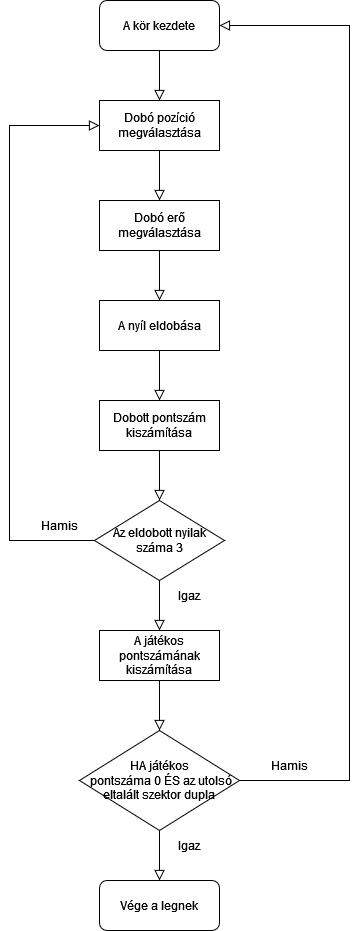
\includegraphics[scale=0.3]{images/darts_flowchart.drawio}
\caption{Darts folyamatábrája}
\label{fig:cimer}
\end{figure}
\begin{itemize}
\item Irodalomkutatás. Amennyiben a dolgozat egy módszer kidolgozására, kifejlesztésére irányul, akkor itt lehet részletesen végignézni (módszertani vagy időrendi bontásban), hogy az eddigiekben milyen eredmények születtek a témakörben.
\item Technológia. Mivel jellemzően kutatásról vagy szoftverfejlesztésről van szó, ezért annak a jellemző elemeit, technikai részleteit itt kell bemutatni.
Ez tehát egy módszeres bevezetés ahhoz, hogy ha valaki nem jártas a témakörben, akkor tudja, hogy a dolgozat milyen aktuálisan elérhető eredményeket, eszközöket használt fel.
\item Piackutatás. Bizonyos témáknál új termék vagy szolgáltatás kifejlesztése a cél.
Ekkor érdemes annak alaposan utánanézni, hogy aktuálisan milyen eszközök érhetők el a piacon.
Ez szoftverek esetében a hasonló alkalmazások bemutatását, táblázatos formában történő összehasonlítását jelentheti.
Szerepelhetnek képek és észrevételek a viszonyításként bemutatott alkalmazásokhoz.
\item Követelmény specifikáció. Külön szakaszban érdemes részletesen kitérni az elkészítendő alkalmazással kapcsolatos követelményekre.
Ehhez tartozhatnak forgatókönyvek (\textit{scenario}-k).
A szemléletesség kedvéért lehet hozzájuk képernyőkép vázlatokat is készíteni, vagy a használati eseteket más módon szemléltetni.
\end{itemize}

\Section{Amit csak említés szintjén érdemes szerepeltetni}

Az olvasóról annyit feltételezhetünk, hogy programozásban valamilyen szinten járatos, és a matematikai alapfogalmakkal sem ebben a dolgozatban kell megismertetni.
A speciális eszközök, programozási nyelvek, matematikai módszerekk és jelölések persze jó, hogy ha említésre kerülnek, de nem kell nagyon belemenni a közismertnek tekinthető dolgokba.
